\chapter{Evaluation on other Techniques}

This chapter will go through some other techniques that could prove to be valuable for the asbestos dataset like the training size of the dataset, different cropping methods, different image augmentations and architectures that have been altered to better meet the underlying tasks' demands.

Data augmentation should add regularization and lead to a model that is better generalizable to the test set. New architectures will then be created to fit better the problem at hand. \\

\section{Evaluation Of Overall Number Of Parameters in VGG13}

Here I want to understand how the overall number of parameters affects the performance of the network. VGG13 was built primarily for the ImageNet Challenge and is probably too big for a task like the asbestos detection. In a first step, I will try to reduce the fully connected layers since they contribute to the complexity of the model the most. I will gradually reduce the number of parameters in the last 3 layers and compare the performance by averaging over 3 runs. Table \ref{tbl:vgg13_fc} shows the results. The last fully connected layer can safely be reduced from initially having 4096 units per layer to 16 units without harming the performance, or even increase it slightly while reducing the overall parameters by 92.39\%. It can be observed that applying transfer learning on a slightly altered architecture quickly diminishes it's advantages as expected. This can be explained because the architecture was relying on a specific configuration. Changing filters or fully connected layers might lead to having to retrain the whole architecture although the drop in performance is surprising for the changes only affect the last fully connected layer of the network. \\


\begin{table}[h] \centering
\ra{1.3}
\caption{Variations in the last 3 fully connected layers of the VGG13 architecture. They were all performed with Batch Normalization. The last columne shows how much parameters remain in the varied architecture relative to the original VGG13 implementation.}
\resizebox{0.9\textwidth}{!}{%
\begin{tabular}{@{}rrrrr@{}}
\toprule & Accuracy (from scratch) & Accuracy (pre-trained) & Number of Parameters & \% of Original \\
\midrule
VGG13\_4096    & 81.0631\% $\pm$ 0.5425 & 88.0398\% $\pm$ 0.7177 & 128'959'042 & 100\% \\
VGG13\_1024    & 80.0664\% $\pm$ 0.7177 & 81.0631\% $\pm$ 0.7177 & 36'153'666 & 28.04\% \\
VGG13\_512    & 80.8416\% $\pm$ 0.7831 & 80.0664\% $\pm$ 0.2713 & 22'520'130 & 17.46\% \\
VGG13\_256    & 80.9524\% $\pm$ 0.8720 & 80.1772 $\pm$ 0.8720 & 15'899'970 & 12.33\% \\
VGG13\_128    & 81.3954\% $\pm$ 0.9781 & 79.7342\% $\pm$ 1.4095 & 12'639'042 & 9.80\% \\
VGG13\_64    & 81.6168\% $\pm$ 0.4144 &  81.1738 \% $\pm$ 0.4144 & 11'020'866 & 8.55\% \\
VGG13\_32    & 80.0665\% $\pm$ 2.3648 & 81.5061 $\pm$ 0.5647 & 10'214'850 & 7.92\% \\
\textbf{VGG13\_16}    & \textbf{82.0598\%} $\pm$ 1.6500 & 79.0697 $\pm$ 0.8138 & 9'812'610 & 7.61\% \\
VGG13\_8    & 78.7375\% $\pm$ 1.5103 & 80.1772 $\pm$ 1.2819 & 9'611'682 & 7.45\% \\
VGG13\_4    & 79.7342\% $\pm$ 0.9781 & 80.1772 $\pm$ 1.9245 & 9'511'266 & 7.38\% \\
VGG13\_2    & 59.8007\% $\pm$ 0.0 & 74.3079 $\pm$ 10.2805 & 9'461'070 & 7.36\% \\
\bottomrule
\end{tabular}}
\label{tbl:vgg13_fc}
\end{table}

As a next step, the fully connected layer is held fixed at the original size of 4096 and the filters of all previous layers are reduced gradually. First, they are all halved until the first layer reaches 16 filters instead of the original 64. Then the layers deeper within the network are halved until all layers have 16 filters. After that configuration is reached all filters all reduced gradually until only 2 filters per layer remain. Table \ref{tbl:vgg_filter_scheme} shows a summary of the filter reduction scheme. The last filter scheme "I" is to see if there is any benefit in increasing filters starting from 2 to the last layer. This imitates the original distribution of the filters but reducing the overall parameters drastically. \\


\begin{table}[H] \centering
\ra{1.3}
\caption{Filter reduction scheme used on the original VGG13 architecture. The fully connected layer at the end is hold fixed and only the intermediate layers are reduced in filter size. The M stands for a max pooling layer.}
\resizebox{0.73\textwidth}{!}{%
\begin{tabular}{@{}rr@{}}
\toprule & VGG13 architecture variations in number of filters\\
\midrule
Original        & [64, 64, M, 128, 128, M, 256, 256, M, 512, 512, M, 512, 512, M]  \\
A                & [32, 32, M, 64, 64, M, 128, 128, M, 256, 256, M, 256, 256, M]  \\
B                & [16, 16, M, 32, 32, M, 64, 64, M, 128, 128, M, 128, 128, M]  \\
C                & [16, 16 M, 16, 16, M, 32, 32, M, 64, 64, M, 64, 64, M]  \\
D                & [16, 16, M, 16, 16, M, 16, 16, M, 32, 32, M, 32, 32, M]  \\
E                & [16, 16, M, 16, 16, M, 16, 16, M, 16, 16, M, 16, 16, M]  \\
F                & [8, 8, M, 8, 8, M, 8, 8, M, 8, 8, M, 8, 8, M]  \\
G                & [4, 4 M, 4, 4, M, 4, 4, M, 4, 4, M, 4, 4, M]  \\
H                & [2, 2, M, 2, 2, M, 2, 2, M, 2, 2, M, 2, 2, M]  \\
I                & [2, 2, M, 4, 4, M, 8, 8, M, 16, 16, M, 32, 32, M]  \\
J                & [2, 2, M, 4, 4, M, 8, 8, M, 16, 16, M, 32, 32, M]  \\
\bottomrule
\end{tabular}}
\label{tbl:vgg_filter_scheme}
\end{table}

The goal is to understand how the filters can be reduced and if a pattern can be observed. The results are summarized in Table \ref{tbl:vgg13_fc}. I can be shown that reducing the filters from the original schema to the scheme "A" does no harm the accuracy but reduces the trainable parameters by roughly 50\%. The standard deviation of 0.2721 gives a rather robust result and is lower than the standard deviation of 0.5425 obtained with the original scheme. Surprising is the result obtained with scheme "G" which uses only 4 filters per each layer reducing the overall parameters by 86.35\%. Although it's worse compared to the original scheme, it suffered only 1.7\% which could be attributed to chance. \\


\begin{table}[h] \centering
\ra{1.3}
\caption{Variations in number of Filters throughout the VGG13 architecture as explained in table \ref{tbl:vgg_filter_scheme}.}
\resizebox{0.9\textwidth}{!}{%
\begin{tabular}{@{}rrrrr@{}}
\toprule & Accuracy (from scratch) & Accuracy (pre-trained) & Number of Parameters & \% of Original \\
\midrule
VGG13\_original    & 81.0631\% $\pm$ 0.5425 & 88.0398\% $\pm$ 0.7177 & 128'959'042 & 100\% \\
VGG13\_a    & 81.0631\% $\pm$ 0.2712 & 74.6401\% $\pm$ 4.4600 & 70'529'186 & 54.69\% \\
VGG13\_b    & 80.3986\% $\pm$ 0.2713 & 80.1771\% $\pm$ 1.8464 & 43'073'874 & 33.40\% \\
VGG13\_c    & 78.7375\% $\pm$ 0.9780 & 80.0664 $\pm$ 0.9780 & 29'790'002 & 23.10\% \\
VGG13\_d    & 79.4020\% $\pm$ 0.8137 & 80.3986\% $\pm$ 0.4698 & 23'261'010 & 18.04\% \\
VGG13\_e    & 78.9590\% $\pm$ 1.0270 &  79.7342 \% $\pm$ 1.8988 & 20'026'514 & 15.53\% \\
VGG13\_f    & 78.7375\% $\pm$ 0.8138 & 79.9557 $\pm$ 0.6826 & 18'404'874 & 14.27\% \\
VGG13\_g    & 79.2913\% $\pm$ 0.6826 & 79.2913 $\pm$ 1.2231 & 17'597'942 & 13.65\% \\
VGG13\_h    & 78.1838\% $\pm$ 0.4143 & 78.6268 $\pm$ 0.5647 & 17'195'448 & 13.33\% \\
\midrule
VGG13\_i    & 79.1805\% $\pm$ 2.2093 & 79.7342 $\pm$ 1.1824 & 23'234'952 & 18.02\% \\
\bottomrule
\end{tabular}}
\label{tbl:vgg13_fc}
\end{table}

Combining both modifications leads to yet another surprise as seen in Table \ref{tbl:vgg13_f_fc}. The modification with only 16 units per fully-connected layer and scheme "D" results in 80.73\% accuracy while reducing the overall complexity of the model by 99.946\%! The time needed to train the model drops from initially 1 hour and 13 minutes to only 25 minutes. But more importantly is that the size of the model is much more deployable for production, e.g. IOT devices. \\


\begin{table}[h] \centering
\ra{1.3}
\caption{Variations in number of Filters throughout the VGG13 architecture as explained in table \ref{tbl:vgg_filter_scheme}.}
\resizebox{0.9\textwidth}{!}{%
\begin{tabular}{@{}rrrrr@{}}
\toprule & Accuracy (from scratch) & run time (hh:mm:ss) & Number of Parameters & \% of Original \\
\midrule
VGG13\_original    & 81.0631\% $\pm$ 0.5425 & 1:13:04 & 128'959'042 & 100\% \\
VGG13\_16\_a            & 80.6201\% $\pm$ 1.2529 & 0:27:01 & 2'556'386 & 1.9823\% \\
VGG13\_16\_b            & 80.6201\% $\pm$ 0.6264 & 0:25:37 & 690'834 & 0.5357\% \\
VGG13\_16\_d            & 80.7309\% $\pm$ 1.4354 & 0:25:35 & 70'290 & 0.0545\% \\
VGG13\_16\_g             & 79.2912\% $\pm$ 1.8061 & 0:25:34 & 4'982 & 0.0039\% \\
\midrule
\bottomrule
\end{tabular}}
\label{tbl:vgg13_f_fc}
\end{table}

Re-optimizing the hyperparameters with SigOpt yielded small improvements as seen in Table \ref{tbl:vgg13_f_fc_optimized}. \\


\begin{table}[h] \centering
\ra{1.3}
\caption{SigOpt opimization VGG13 architecture as explained in table \ref{tbl:vgg_filter_scheme}.}
\resizebox{0.9\textwidth}{!}{%
\begin{tabular}{@{}rrrrr@{}}
\toprule & Accuracy (from scratch) & run time (hh:mm:ss) & Number of Parameters & \% of Original \\
\midrule
VGG13\_original    & 81.0631\% $\pm$ 0.5425 & 1:13:04 & 128'959'042 & 100\% \\
VGG13\_16\_d            & 81.2846\% $\pm$ 1.0963 & 0:25:34 & 70'290 & 0.0545\% \\
VGG13\_16\_g             & 80.0664\% $\pm$ 0.4698& 0:25:08 & 4'982 & 0.0039\% \\
\midrule
\bottomrule
\end{tabular}}
\label{tbl:vgg13_f_fc_optimized}
\end{table}

\subsection{Visualization of VGG}

First lets visualize the architecture with the best results obtained which is the pre-trained vgg13 model with batch normalization. The GradCam was taken on the last convolutional layer and can be seen in Figure \ref{fig:asbestos_gradcam}. On the 

\begin{figure}[H]
\centering
\caption{GradCam visualization applied on the left image once with looking for asbestos structures (right) and once looking for not-asbestos structures (middle).}
\subfigure{
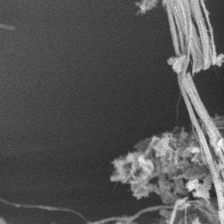
\includegraphics[width=.3\textwidth]{images/chapter6/vgg13/asbestos-original.png}
}
\subfigure{
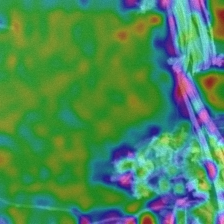
\includegraphics[width=.3\textwidth]{images/chapter6/vgg13/asbestos-gradcam-0.png}
}
\subfigure{
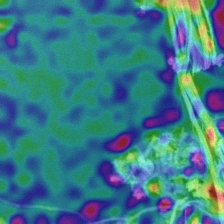
\includegraphics[width=.3\textwidth]{images/chapter6/vgg13/asbestos-gradcam-1.png}
}
\label{fig:asbestos_gradcam}
\end{figure}

Visualizing images that activate certain filters in the last layer maximally are seen in Figure \ref{fig:vgg13_filter_activation}. The images are very similar to the visualizations on ImageNet with structures that do not resemble asbestos at all. Nontheless they achieve the best performance so far. I argue that some filter from ImageNet do indeed capture another structure in real life that resembels that of asbestos fibers, and if these very few filters are activated strongly. The classification in the end is done on these very few filters and the rest (the majority) is ignored. That's why reducing the last fully-connected layer to 16 does not harm the performance at all.

\begin{figure}[H]
\centering
\caption{Last Layer visualizations (8 of 512) of the pre-trained VGG13 with batch normalization.}
\subfigure{

\includegraphics[width=.23\textwidth]{images/chapter6/vgg13/layers-pretrained/l22-f1.jpg}
}
\subfigure{

\includegraphics[width=.23\textwidth]{images/chapter6/vgg13/layers-pretrained/l22-f2.jpg}
}
\subfigure{
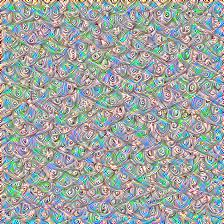
\includegraphics[width=.23\textwidth]{images/chapter6/vgg13/layers-pretrained/l22-f3.jpg}
}
\subfigure{
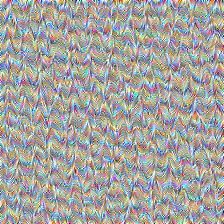
\includegraphics[width=.23\textwidth]{images/chapter6/vgg13/layers-pretrained/l22-f4.jpg}
}
\subfigure{
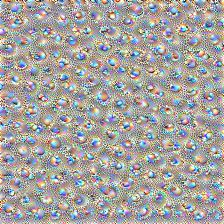
\includegraphics[width=.23\textwidth]{images/chapter6/vgg13/layers-pretrained/l22-f5.jpg}
}
\subfigure{
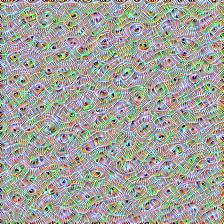
\includegraphics[width=.23\textwidth]{images/chapter6/vgg13/layers-pretrained/l22-f6.jpg}
}
\subfigure{
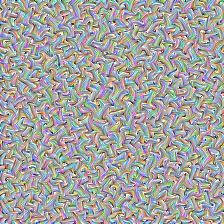
\includegraphics[width=.23\textwidth]{images/chapter6/vgg13/layers-pretrained/l22-f7.jpg}
}
\subfigure{

\includegraphics[width=.23\textwidth]{images/chapter6/vgg13/layers-pretrained/l22-f8.jpg}
}
\label{fig:vgg13_filter_activation}
\end{figure}

As oposed to the VGG13 architecture modification with scheme "G" and only 16 units in the fully connected layers. Here all the four filters are shown from the last layer. They don't resemble neither the ImageNet filters, nor something that resembels asbestos.

\begin{figure}[H]
\centering
\caption{GradCam visualization applied on the left image once with looking for asbestos structures (right) and once looking for not-asbestos structures (middle).}
\subfigure{
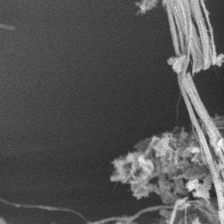
\includegraphics[width=.3\textwidth]{images/chapter6/vgg13/asbestos-original.png}
}
\subfigure{
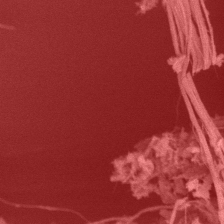
\includegraphics[width=.3\textwidth]{images/chapter6/vgg13/layers-g-16/gradcam0.png}
}
\subfigure{
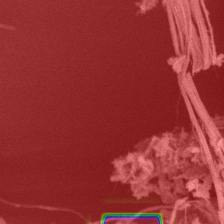
\includegraphics[width=.3\textwidth]{images/chapter6/vgg13/layers-g-16/gradcam1.png}
}
\label{fig:asbestos_gradcam}
\end{figure}


\begin{figure}[H]
\centering
\caption{Last Layer visualizations (8 of 512) of the pre-trained VGG13 with batch normalization.}
\subfigure{
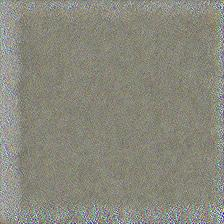
\includegraphics[width=.23\textwidth]{images/chapter6/vgg13/layers-g-16/l22-f0.jpg}
}
\subfigure{

\includegraphics[width=.23\textwidth]{images/chapter6/vgg13/layers-g-16/l22-f1.jpg}
}
\subfigure{

\includegraphics[width=.23\textwidth]{images/chapter6/vgg13/layers-g-16/l22-f2.jpg}
}
\subfigure{
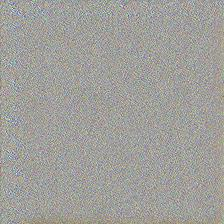
\includegraphics[width=.23\textwidth]{images/chapter6/vgg13/layers-g-16/l22-f3.jpg}
}
\label{fig:asbestos_gradcam}
\end{figure}

\section{Evaluation Of Different Dataset Sizes And Variations}

All the different dataset variations are compared against each other within the same architecture. Each result is obtained by running the model three times and averaging over all runs. Table \ref{tbl:resnet18_dataset} shows the results for ResNet18

\begin{table}[h] \centering
\ra{1.3}
\caption{Dataset variations with ResNet18. The first group shows how the datasets performed when trained from scratch whereas the second group shows how the datasets performed with pre-training.}
\resizebox{0.79\textwidth}{!}{%
\begin{tabular}{@{}rrrr@{}}
\toprule & accuracy (from scratch) & accuracy (pre-trained) &   $\Delta$ \\
\midrule
FINAL                        & 79.62\%  $\pm$ 0.9465 &   86.93\% $\pm$ 0.7757   & -     \\
FINAL\_C                    &     80.73\% $\pm$ 0.3839 &     84.05\% $\pm$  0.9584 & - \\
FINAL\_C\_B                &     81.39\% $\pm$ 1.3827 &     85.27\% $\pm$  0.7988 & - \\
FINAL\_CH                    &     81.62\% $\pm$ 0.2942 &     84.94\% $\pm$  0.3966 & - \\
FINAL\_CH\_B                &     80.73\% $\pm$ 0.8371 &     85.05\% $\pm$  0.3300 & - \\
FINAL\_EXTENDED        &     81.06\% $\pm$ 0.3839 &     84.5\% $\pm$ 0.8649 & - \\
\bottomrule
\end{tabular}}
\label{tbl:resnet18_dataset}
\end{table}

Changing the train set by reducing questionable and unclear images has lead to consistent improvements in the ResNet18 model trained from scratch but to consistently worse results when training from pre-trained weights. [QUESTION: maybe that shows that training from scratch needs better quality images while training from a checkpoint is less sensitive to wrong images but needs more images. I don't think that's true though....]. In Table \ref{fig:densenet121_dataset} the summary shows how DenseNet121 reacts with different datasets.

\begin{table}[h] \centering
\ra{1.3}
\caption{Dataset variations with DenseNet121. The first group shows how the datasets performed when trained from scratch whereas the second group shows how the datasets performed with pre-training.}
\resizebox{0.79\textwidth}{!}{%
\begin{tabular}{@{}rrrr@{}}
\toprule & accuracy (from scratch) & accuracy (pre-trained) &   $\Delta$ \\
\midrule
FINAL                        & 83.72\%  $\pm$ 1.1963 &   86.16\% $\pm$ 1.1704   & -     \\
FINAL\_C                    &     82.61\% $\pm$ 0.9678 &     83.94\% $\pm$  0.5852 & - \\
FINAL\_C\_B                &     80.39\% $\pm$ 0.3840 &     85.38\% $\pm$  0.1905 & - \\
FINAL\_CH                    &     79.61\% $\pm$ 2.2322 &     86.60\% $\pm$  0.3998 & - \\
FINAL\_CH\_B                &     83.17\% $\pm$ 0.1100 & 81.775\% $\pm$  3.3806 & - \\
FINAL\_EXTENDED        &     83.06\% $\pm$ 1.0169 &     85.60\% $\pm$ 2.1218 & - \\
\bottomrule
\end{tabular}}
\label{tbl:densenet121_dataset}
\end{table}

With Densenet121 there is no improvement to be seen by changing the dataset. If trained from scratch all variations lead to worse results. If trained with pre-trained weights, the FINAL\_CH dataset yields marginally better accuracy but that is most certainly due to chance. In Table \ref{fig:inceptionv3_dataset} the summary shows how Inception v3 behaves with different datasets.

\begin{table}[h] \centering
\ra{1.3}
\caption{Dataset variations with Inception v3. The first group shows how the datasets performed when trained from scratch whereas the second group shows how the datasets performed with pre-training. FINAL\_C\_B died for the non-pre-trained twice. Only one datapoint used.}
\resizebox{0.79\textwidth}{!}{%
\begin{tabular}{@{}rrrr@{}}
\toprule & accuracy (from scratch) & accuracy (pre-trained) &   $\Delta$ \\
\midrule
FINAL                        & 82.83\%  $\pm$ 0.6157 &  85.93\% $\pm$ 0.3998   & -     \\
FINAL\_C                    &     80.4\% $\pm$ 0.6926 & 85.82\% $\pm$  0.2942 & - \\
FINAL\_C\_B                &     82.06\% $\pm$ 0.0\* & 83.83\% $\pm$  0.3989 & - \\
FINAL\_CH                    &     ?\% $\pm$ ? &     ?\% $\pm$ ? & - \\
FINAL\_CH\_B                &     81.06\% $\pm$ 0.3839 & 85.27\% $\pm$  1.2200 & - \\
FINAL\_EXTENDED        &     81.72\% $\pm$ 0.3839 &     84.16\% $\pm$ 0.4433 & - \\
\bottomrule
\end{tabular}}
\label{tbl:inceptionv3_dataset}
\end{table}

Inception v3 died several times during testing so the data points are not complete. But in general it shows the same behavior as with the other two architectures, there is no improvement by changing the dataset. Also surprising is the fact that FINAL\_EXTENDED yielded better results for ResNet18 trained from scratch only. All other runs resulted in a worse overall accuracy which is difficult to understand.

\section{Evaluation Of Different Cropping And Augmentation Methods}

\subsection{FiveCrop}

The torch library already had a FiveCrop implementation which could be used with minor changes in the code. The FiveCrop implementation crops 5 images of a given size from the whole image. All corners and the center are cropped. In training and evaluation, these crops are stacked on top of each other and then the average per pixel is computed.

Table XXX summarizes the results.

\begin{table}[h] \centering
\ra{1.3}
\caption{Resnet18 FiveCrop Implementation with and without pre-training. FINAL (regular) means ResNet18 with the resizing of the image instead of cropping and averaging}
\resizebox{0.79\textwidth}{!}{%
\begin{tabular}{@{}rrrr@{}}
\toprule & accuracy (from scratch) & accuracy (pre-trained) &   $\Delta$ \\
\midrule
FINAL (regular)                & 79.62\%  $\pm$ 0.9465 &   86.93\% $\pm$ 0.7757   & -     \\
FINAL (fiveCrop)            & 83.72\% &  87.04\%   & -     \\
\bottomrule
\end{tabular}}
\label{tbl:resnet18-fivecrop}
\end{table}

\subsection{RandomNineCrop}

The torch library already had a FiveCrop implementation which could be used with minor changes in the code. The FiveCrop implementation crops 5 images of a given size from the whole image. All corners and the center are cropped. In training and evaluation, these crops are stacked on top of each other and then the average per pixel is computed.

Table XXX summarizes the results.

\begin{table}[h] \centering
\ra{1.3}
\caption{Resnet18 FiveCrop Implementation with and without pre-training. FINAL (regular) means ResNet18 with the resizing of the image instead of cropping and averaging}
\resizebox{0.79\textwidth}{!}{%
\begin{tabular}{@{}rrrr@{}}
\toprule & accuracy (from scratch) & accuracy (pre-trained) &   $\Delta$ \\
\midrule
FINAL (regular)                & 79.62\%  $\pm$ 0.9465 &   86.93\% $\pm$ 0.7757   & -     \\
FINAL (randomNine)            & 83.39\% &  88.04\%   & -     \\
\bottomrule
\end{tabular}}
\label{tbl:resnet18-randomnine}
\end{table}

\section{Reducing the Number of Filters}

The current architectures used for this thesis are all huge with parameters ranging from XX million to XX million. They were originally built to classify a variety of different objects found in ImageNet. Not only object as cars and dogs needed to be distinguished but also different and sometimes similar breeds of dogs. Thus it makes sense to learn hundreds of new feature mappings for each layer of the network. With the asbestos task at hand, it might be different and a few filters per layer could possibly suffice. That is not to say, that the task is simple in its nature, but that asbestos has a common looking structure and the networks hard work is to find this structure in many different settings and under difficult conditions. Reducing the number of filters has another huge benefit of reducing the overall number of trainable parameters and thus speeding up the learning process, using less memory and being much easier to deploy on productive configurations.\\

For the above-mentioned reason, the ResNet18 implementation has been altered to contain only a certain amount of filters in each single layer. The amount has been set to different values ranging from 1 to 32 filters. With 32 filters of size 3x3 only 320 parameters are used per layer. In ResNet18, for example, there are 4 blocks of 2 layers of 320 parameters making in total 2560 parameters. That does not yet count in the first 7x7 convolution and the fully-connected layer with its softmax function but the number of parameters is reduced dramatically as shown in Table XXXX.


\begin{table}[h] \centering
\ra{1.3}
\caption{Resnet18 with different number of filters on the FINAL dataset. The number of filters present in paranthesis is the number of filters used per layer.}
\resizebox{0.79\textwidth}{!}{%
\begin{tabular}{@{}rrrrr@{}}
\toprule & accuracy (from scratch) & trainable parameters &  param reduction (\%) \\
\midrule
ResNet18 (official)            & 79.62\% &  11'177'538 & -     \\
ResNet18 (32 filters)            & 78.405\% &  156'578 & -     \\
ResNet18 (16 filters)            & 81.06\% &  40'658 & -     \\
ResNet18 (8 filters)            & 79.402\% &  10'922 & -     \\
ResNet18 (4 filters)            & 79.62\% &  3'110 & -     \\
ResNet18 (2 filters)            & 80.066\% &  968 & -     \\
ResNet18 (1 filter)                & 75.083\% &  338 & -     \\

\bottomrule
\end{tabular}}
\label{tbl:resnet18-sixteen}
\end{table}

The problem here is that I went several ways... sometimes by reduced filter size then I increased batch size and input size.... I guess I will do many subchapters for this or split the evaluation into 2 parts... evaluation regarding transfer learning and evaluation regarding my own architectures.

\section{Evaluation of Different Image Size Inputs to the network}

\begin{table}[h] \centering
\ra{1.3}
\caption{Resnet18 FiveCrop Implementation with and without pre-training. FINAL (regular) means ResNet18 with the resizing of the image instead of cropping and averaging}
\resizebox{0.79\textwidth}{!}{%
\begin{tabular}{@{}rrrr@{}}
\toprule & accuracy (from scratch) & accuracy (pre-trained) &   $\Delta$ \\
\midrule
FINAL (regular 224)                & 79.62\%  $\pm$ 0.9465 &   86.93\% $\pm$ 0.7757   & -     \\
FINAL (input 448)            & 76.74\% &  -   & -     \\
\bottomrule
\end{tabular}}
\label{tbl:resnet18-448}
\end{table}

\begin{table}[h] \centering
\ra{1.3}
\caption{Resnet18 FiveCrop Implementation with and without pre-training. FINAL (regular) means ResNet18 with the resizing of the image instead of cropping and averaging}
\resizebox{0.79\textwidth}{!}{%
\begin{tabular}{@{}rrrr@{}}
\toprule & accuracy (from scratch) & accuracy (pre-trained) &   $\Delta$ \\
\midrule
FINAL (regular 224)                & 79.62\%  $\pm$ 0.9465 &   86.93\% $\pm$ 0.7757   & -     \\
FINAL (input 448)            & 76.74\% &  -   & -     \\
FINAL (input 896)            & 78.74\% &  -   & -     \\
FINAL (input 1024)            & 80.40\% &  -   & -     \\
\bottomrule
\end{tabular}}
\label{tbl:resnet18-896}
\end{table}


\begin{table}[h] \centering
\ra{1.3}
\caption{Resnet18 FiveCrop Implementation with and without pre-training. FINAL (regular) means ResNet18 with the resizing of the image instead of cropping and averaging}
\resizebox{0.79\textwidth}{!}{%
\begin{tabular}{@{}rrrr@{}}
\toprule & accuracy (from scratch) & accuracy (pre-trained) &   $\Delta$ \\
\midrule
FINAL (regular 224)                & 79.62\%  $\pm$ 0.9465 &   86.93\% $\pm$ 0.7757   & -     \\
FINAL (input 1024)            & 80.40\% &  -   & -     \\
\bottomrule
\end{tabular}}
\label{tbl:resnet18-1024}
\end{table}

\section{Evaluation of Smaller and more Restrictive Training Data}